\documentclass[11pt,a4paper,twocolumn]{article}

\usepackage{amsfonts}
\usepackage{amsmath}
\usepackage{geometry}
\usepackage{xcolor,graphicx}
\usepackage[subfolder,cleanup]{gnuplottex}
%\usepackage{amsthm}
%\usepackage{enumitem}
%\usepackage{wrapfig}
\usepackage{subcaption}
%\usepackage{hyperref}
\usepackage{tikz}
\usepackage{stfloats}

\usepackage{lipsum}

\usetikzlibrary{%
	decorations.pathreplacing,%
 	decorations.pathmorphing%
}

%\usepackage[table]{xcolor}
%\rowcolors{2}{gray!25}{white}

\let\originalleft\left
\let\originalright\right
\renewcommand{\left}{\mathopen{}\mathclose\bgroup\originalleft}
\renewcommand{\right}{\aftergroup\egroup\originalright}


\renewcommand\bottomfraction{.8}

\newcommand{\df}{\, \textrm{d}}
\newcommand{\e}{\textrm{e}}
\newcommand{\diff}[3][]{\frac{\df^{#1}#2}{\df{#3}^{#1}}}
\newcommand{\pdiff}[3][]{\frac{\partial^{#1}#2}{\partial{#3}^{#1}}}
\newcommand{\eps}{\varepsilon}
\providecommand{\bigO}[1]{\ensuremath{\mathop{}\mathopen{}\mathcal{O}\mathopen{}\left(#1\right)}}

\definecolor{Beer}{HTML}{FFCC00}

\bibliographystyle{ieeetr}

\title{The Dynamics of Spilled Beer}
\author{Brady Metherall}
\date{11 November 2019}

\newgeometry{margin=2cm}
%\setlength\parindent{0pt}

\begin{document}
\maketitle


\setlength{\belowdisplayskip}{6.5pt} \setlength{\belowdisplayshortskip}{6.5pt}
\setlength{\abovedisplayskip}{6.5pt} \setlength{\abovedisplayshortskip}{6.5pt}


\section{Introduction}
\begin{figure}[tbp]
\centering
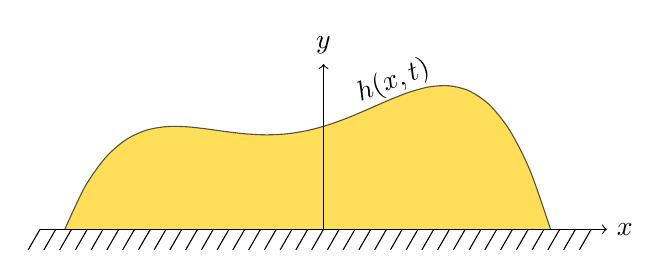
\begin{tikzpicture}[scale=0.6]
% Beer outline
\draw [scale=4,domain=-1.36921:1.20148,smooth,variable=\x,fill=Beer,opacity=0.65] plot ({\x)},{0.5 * (1 - (\x*\x - 1) * (\x + 3/10)^2)});
% Label
\node at (1.6,4*0.7058) [anchor=south,rotate=21.4,yshift=-1mm] {$h(x,t)$};
% Table
\draw [->] (-6,0) -- (6,0) node [right] {$x$};
\draw [decorate,decoration={border,angle=-120,amplitude=3mm,segment length=2mm}] (-6,0) -- (6,0);
% y axis
\draw [->] (0,0) -- (0,3.5) node [above] {$y$};
\end{tikzpicture}
\caption{Beer spilled on a table.}
\label{fig:beer}
\end{figure}

We seek to determine the dynamics of a small puddle of beer spilled on a table as in Figure \ref{fig:beer}. Of particular interest is the height and shape of the beer, $h$, as it spreads, as well as the amount of time we'd have to move out of the way of the beer as it runs down an angled table. To model the scenario we begin with the Navier-Stokes equation,
\begin{align}
\rho \left( \mathbf{u}_t + \left( \mathbf{u} \cdot \nabla \right) \mathbf{u} \right) &= - \nabla p + \mu \nabla^2 \mathbf{u} + \rho \mathbf{g},
\label{eq:ns}
\end{align}
and derive equations of by so-called lubrication theory. Lubrication theory deals with fluid flow in which the length scale of one dimension is considerably less than the rest, for example, lubricated bearings in machinery. In the context of beer spilled into a table, we shall assume the height of the droplet is substantially smaller than the girth. Let us define the parameter $\eps \ll 1$ to be this ratio, that is, $\eps := H L^{-1}$, where $H$ is the characteristic height, and $L$ the characteristic length.

In Section \ref{sec:flat} we shall non-dimensionalize \eqref{eq:ns} and perform rudimentary asymptotic analysis. This will give us a greatly simplified system which we can solve analytically in multiple geometries---including cartesian and cylindrical. We shall then repeat our analysis in Section \ref{sec:angled} for the more general case of an angled table, and analyse the profile of the spill as it travels down the table.

\section{Flat Table}
\label{sec:flat}
We begin by non-dimensionalizing \eqref{eq:ns} by scaling time by $L$ divided by the characteristic fluid speed, the pressure as hydrostatic, and by assuming the fluid motion is driven by the pressure gradient \cite{howison}. This yields
\begin{align}
\nonumber \text{Re}' \left( u_t + u \, u_x + v \, u_y \right) &= - p_x + \eps^2 u_{xx} + u_{yy}, \\
\text{Re}' \eps^2 \left( v_t + u \, v_x + v \, v_y \right) &= \\
\nonumber - p_y &+ \eps^4 v_{xx} + \eps^2 v_{yy} - 1,
\end{align}
for the $x$ and $y$ components, respectively, where Re$'$ is the reduced Reynolds number. To leading order we obtain
\begin{align}
\bigO{1} \colon \ p_x &= u_{yy}, & \bigO{1} \colon \ p_y &= -1.
\end{align}
After imposing the boundary conditions that $u = 0$ on $x = 0$, and $u_y = 0$ on $y = h$, we~find
\begin{align}
u = -\frac{1}{2} \left( 2hy - y^2 \right) h_x.
\end{align}

We can now readily find the flux of the flow, and therefore, develop a conservation equation. The mass flux is given as the flow of the fluid multiplied by its velocity---that is, the flux is $\int_0^h u \df y$. Despite the analysis thus far having been in two dimensions, the $z$ direction behaves exactly as the $x$ direction. Therefore, we can write conservation of mass as
\begin{align}
h_t = \frac{1}{3} \nabla \cdot \left( h^3 \nabla h \right),
\label{eq:height}
\end{align}
subject to
\begin{align}
\int_{\mathbb{R}^n} h \df^n x = 1
\label{eq:int}
\end{align}
for all times $t$.

\subsection{Two Dimensional Case}
Proceeding with a self-similar solution \cite{zwillinger}, \eqref{eq:height} can be solved in two dimensions. If we assume $h$ has the form $h(x,t) = t^\alpha f(\eta)$ where $\eta = x t^{-\beta}$, we find \eqref{eq:height} and \eqref{eq:int} depend only on $\eta$ for $\alpha = -1/5$ and $\beta = 1/5$. This leads us to the ordinary differential equation
\begin{align}
 \left( f^3 f \right)' = \frac{-3}{5} \left( \eta f' + f \right).
\end{align}
Solving this yields
\begin{align}
f =
\begin{cases}
\left( \frac{9}{10} \right)^{1/3} \left( \eta_*^2 - \eta^2 \right)^{1/3} & |\eta| \leq \eta_* \\
0 & \text{otherwise}
\end{cases},
\end{align}
where
\begin{align}
\eta_* &= \left( \frac{6075 \Gamma^6 \left( \frac{2}{3} \right) \Gamma^6 \left( \frac{11}{6} \right)}{16 \pi^9} \right)^{1/10} \approx 0.747412
\end{align}
is the finite extent of the droplet---found from~\eqref{eq:int}~\cite{gradshteyn}. This solution can be seen in Figure~\ref{fig:2ddrop}.

\begin{figure*}[tbp]
\centering
\begin{subfigure}{0.5\textwidth}
\centering
\begin{gnuplot}[terminal=epslatex, terminaloptions={color size 3.2in,1.75in lw 3}]
set grid
set format x '%.1f'
set format y '%.2f'
set xl '$x t^{-1/5}$'
set yl '$t^{1/5} h(x,t)$'
set ytics 0.25
set xr [-1:1]
set yr [0:1]
set size ratio -1
p 'Cartesian.dat' u 1:2 w l not
\end{gnuplot}
\caption{Two dimensional.}
\label{fig:2ddrop}
\end{subfigure}%
\begin{subfigure}{0.5\textwidth}
\centering
\begin{gnuplot}[terminal=epslatex, terminaloptions={color size 3.2in,1.75in lw 3}]
set grid
set format x '%.1f'
set format y '%.2f'
set xl '$r t^{-1/8}$'
set yl '$t^{1/4} h(r,t)$'
set ytics 0.25
set xr [-1:1]
set yr [0:1]
set size ratio -1
p 'Polar.dat' u 1:2 w l not
\end{gnuplot}
\caption{Radially symmetric. }
\label{fig:raddrop}
\end{subfigure}
\caption{Self-similar solution to \eqref{eq:height} subject to \eqref{eq:int}.}
\label{fig:selfsim}
\end{figure*}

\subsection{Radially Symmetric Case}
We now instead assume the droplet is in three dimensions, but is radially symmetric. As with the previous subsection, we seek a self-similar solution of the form $h(r,t) = t^\alpha f(\eta)$ where $\eta = r t^{-\beta}$. In this case we find $\alpha = -1/4$ and $\beta = 1/8$, and obtain the ordinary differential equation
\begin{align}
\left( \eta f^3 f' \right)' = \frac{-3}{8} \left( 2 \eta f + \eta^2 f' \right). 
\end{align}
We find the solution
\begin{align}
f =
\begin{cases}
 \left( \frac{9}{16} \right)^{1/3} \left( \eta_*^2 - \eta^2 \right)^{1/3} & |\eta| \leq \eta_* \\
0 & \text{otherwise}
\end{cases}
\end{align}
in this situation---comparable to the two dimensional case---where, similarly,
\begin{align}
\eta_* &= \left( \frac{1024}{243 \pi^3} \right)^{1/8} \approx 0.779212
\end{align}
is the extent of the droplet. This solution can be seen in Figure \ref{fig:raddrop}.

\section{Angled Table}
\label{sec:angled}

\begin{figure}[bp]
\centering
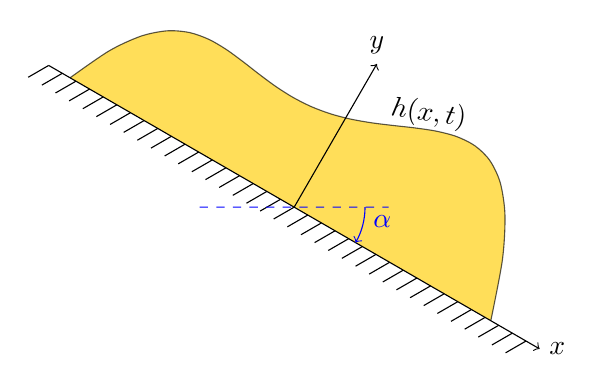
\begin{tikzpicture}[auto,rotate=-30,scale=0.6]
% Beer outline
\draw [scale=4,domain=-1.36921:1.20148,smooth,variable=\x,fill=Beer,opacity=0.65] plot ({\x)},{0.5 * (1 - (\x*\x - 1) * (\x + 3/10)^2)});
% Label
\node at (1.6,4*0.7058) [anchor=south,rotate=21.4-30,yshift=-1mm] {$h(x,t)$};
% Table
\draw [->] (-6,0) -- (6,0) node [right] {$x$};
\draw [decorate,decoration={border,angle=-120,amplitude=3mm,segment length=2mm}] (-6,0) -- (6,0);
% y axis
\draw [->] (0,0) -- (0,3.5) node [above] {$y$};
% Angle
\draw [dashed,blue] (-2*0.866,-1) -- (2*0.866,1);
\draw [<-,blue] (1.5,0) arc (0:30:1.5) node [pos=0.6,anchor=west] {$\alpha$};
\end{tikzpicture}
\caption{Beer droplet spilled on a significantly angled table.}
\label{fig:tilted}
\end{figure}

In this section we shall perform a similar analysis as in the previous section, however, we suppose the table is at considerable angle, $\alpha$, from horizontal. This new scenario is depicted in Figure \ref{fig:tilted}. Due to this angle, we modify the assumption that the motion is driven by the pressure gradient so that gravity is the driving force \cite{howison}. This difference~yields
\begin{equation}
\begin{aligned}
\text{Re}' \left( u_t + u \, u_x + v \, u_y \right) &= \\
- \eps p_x + &\eps^2 u_{xx} + u_{yy} + \sin \alpha, \\
\text{Re}' \eps \left( v_t + u \, v_x + v \, v_y \right) &= \\
- p_y + &\eps^3 v_{xx} + \eps v_{yy} - \cos \alpha,
\end{aligned}
\end{equation}
for the $x$ and $y$ components, respectively. Once again, to leading order we find
\begin{align}
\bigO{1} \colon \> u_{yy} &= - \sin \alpha, & \bigO{1} \colon \> p_y &= - \cos \alpha.
\end{align}
In a similar manner as the previous section, we discover
\begin{align}
u = \frac{1}{2} \sin \alpha \left( 2hy - y^2 \right),
\end{align}
and mass conservation becomes
\begin{align}
h_t + \frac{1}{3} \sin \alpha (h^3)_x = 0.
\label{eq:char}
\end{align}
The partial derivative with respect to $x$ can be expanded to give a quasi-linear partial differential equation. To solve such an equation we proceed using the method of characteristics \cite{zwillinger}. For simplicity we take the boxcar function,
\begin{align}
h_0(x) =
\begin{cases}
1 & |x| \leq \frac{1}{2} \\
0 & \text{otherwise}
\end{cases},
\label{eq:ic}
\end{align}
to be the initial condition---a crude representation of an initial spill of beer.



\begin{figure}[tbp]
\vspace{-5mm}
\begin{gnuplot}[terminal=epslatex, terminaloptions={color size 3in,2.25in lw 3}]
load './Blues.p'

set grid front
set format x '%.1f'
set format y '%.0f'
set format cb '%.1f'
set xr [-1:1.5]
set ytics 2

set xl '$x$'
set yl rotate by 0 '$t$'
set cbl '$h(x,t)$'

set view map

set label 1 'I' at -0.75, 2.92 front center
set label 2 'II' at 0.25, 0.67 front center
set label 3 'III' at 1.25, 2.92 front center
set label 4 'IV' at 0.25, 2.92 front center

sp 'Char.dat' u 1:2:3 w image not, \
'Edges.dat' u 7:8:(0) w l dt 3 lc 8 lw 0.5 not, \
'Edges.dat' u 1:2:(0) w l lc 8 not, \
'Edges.dat' u 3:4:(0) w l lc 8 not, \
'Edges.dat' u 5:6:(0) w l lc 8 not, \
'Shock2.dat' u 1:2:(0) w l lc 8 not
\end{gnuplot}
\vspace{-1.2mm}
\caption{Density plot of the solution of \eqref{eq:char} subject to \eqref{eq:ic} with $\alpha = \pi / 6$. Regions I and III are the trailing and leading edge of the spill, respectively, and therefore, $h=0$. Region II has a constant height of 1 as the spill initially moves downward along the table. Finally, region IV is a rarefaction fan caused by the no-slip condition. The thin dotted line in the upper portion of region III is to highlight the fact that the boundary begins to curve as the fan begins to interact with the shock.}
\label{fig:char}
\end{figure}

The solution of this system can be seen in Figure~\ref{fig:char}. The height of the spill within the rarefaction fan (region IV of Figure \ref{fig:char}) is found to be
\begin{align}
h &= \left( \frac{x + \frac{1}{2}}{t \sin \alpha} \right)^{1/2}.
\end{align}
Furthermore, by the Rankine--Hugoniot condition~\cite{zwillinger} we determine the behaviour of the shock at the interface of the spill to be
\begin{align}
\sigma(t) =
\begin{cases}
\frac{1}{2} + \frac{1}{3} \sin \alpha t & 0 \leq t \leq \frac{3}{2} \csc \alpha \\
\left( \frac{9 t \sin \alpha}{4} \right)^{1/3} - \frac{1}{2} & \frac{3}{2} \csc \alpha \leq t
\end{cases}.
\label{eq:shock}
\end{align}

\begin{figure}[tbp]
\centering
\begin{gnuplot}[terminal=epslatex, terminaloptions={color size 3.2in,2in lw 3}]
set grid
set format x '%.0f'
set format y '%.1f'

set xtics 3
set ytics 0.5

set xr [0:15]
set yr [0:2]

set xl '$t$'
set yl rotate '$\frac{1}{3} \sin \alpha h^3 \enspace \left( \times 10^{-1} \right)$'

p 'Flow.dat' u 1:(10*$2) w l t '$x = 0.6$', \
'Flow.dat' u 1:(10*$3) w l t '$x = 1.0$' dt 2, \
'Flow.dat' u 1:(10*$4) w l t '$x = 1.4$' dt 5
\end{gnuplot}
\caption{Flow rate for various positions, $x$, for $\alpha~=~\pi / 6$.}
\label{fig:flow}
\end{figure}

With the dynamics fully determined, we are now able to investigate the nature of the solution. In the context of spilling beer on an angled table, we are most interested in how much time we'd have to move out of the path of the beer, and---failing to do so---how wet we would become. The (non-dimensional) time we have to avoid the spill is simply the time at which the shock reaches the edge of the table given by \eqref{eq:shock}. To establish the flow rate---and thus, how wet we would become---we must return to the conservative law, \eqref{eq:char}. The flow rate is equivalent to the flux: $\sin \alpha h^3 / 3$. This is shown for three table lengths in Figure \ref{fig:flow}. If you are insufficiently fast, and take $T$ time to move away from the trajectory of the beer, you will soon---unfortunately---find $\int_0^T \sin \alpha h^3 / 3 \df t$ beer in your lap.

\section{Conclusion}
By non-dimensionalizing the Navier-Stokes equation using the ideas of lubrication theory, we developed a mathematical model for the evolution of a small spill of beer on a table. We investigated for the case of a two dimensional beer spill, as well as a radially symmetric spill by finding the self-similar shape. We then extended our model to a table that is sloped at an appreciable angle. In this case we rederived the model to take into account that the flow was dominated by gravity instead of by pressure. Finally, we found how the shape of the droplet transforms as it moves down the table, and how much time an unlikely individual at the end of the table would have to move out of the way to avoid getting wet.

\bibliography{Ref}

\end{document}
